\documentclass{article}
\usepackage{graphicx}
\usepackage{caption}
\usepackage[ngerman]{babel}

\begin{document}

\title{Aufgaben 2 \& 3 - Objektvermessung in \textit{OpenCV-Python} \\
		\large Computer Vision \\
    		Hochschule Darmstadt, Sommersemester 2020}

\author{Roman Kessler}

\maketitle








In der vorliegenden Arbeit wird beschrieben, wie Objekte in \textit{OpenCV-Python} \textit{[Brad00][OpenCV]} vermessen werden können. Das Vorgehen ist eine von mehreren Möglichkeiten, und orientiert sich an den in der Praktikumsaufgabe vorgegebenen Schritten. Ziel ist es, mit Hilfe eines Referenzobjektes $R$ mit bekannter Größe, die unbekannten Größen der Testobjekte $P_{i}$ zu bestimmen. Als $R$ habe ich mich für ein kleines Lineal entschieden (Abb. \ref{fig:fig1}). Als $P_{1}$ dient ein Imbusschlüssel (Abb. \ref{fig:fig2}), und als $P_{2}$ ein Bierdeckel (Abb. \ref{fig:fig3}).

\section{Vorüberlegungen \& Bildakquisition}

Als Referenzobjekt wurde ein Lineal ausgewählt, welches eine Kante mit einer definierten Länge von $120mm$ aufweist. Wir möchten mit Hilfe von $R$ einen Faktor zur Umrechnung von Pixel in das metrische System erhalten. Hier war ein Gedanke, ein möglichst großes $R$ auszuwählen. Das hat den Vorteil, dass der analoge Messfehler beim Messen des großen $R$ (in diesem Fall Ablesen der Skala) proportional zur Objektgröße geringer ist, und somit nicht so stark ins Gewicht fallen wird bei der Bestimmung des Umrechnungsfaktors zwischen Pixel und Millimeter (siehe \ref{laengenber}). $P_{1}$ wurde in der Aufgabe vorgegeben, und $P_{2}$ wurde ausgewählt, um die Objektvermessung an wohldefinierten Kanten, wie den Kanten des Schriftzuges in $P_{2}$ zu testen.

Alle Objekte wurden auf einem weisen, möglichst homogenen Hintergrund platziert, und in einem ungefähren Winkel von $90^{\circ}$ fotografiert, um wenig Verfälschung der Größen durch die Perspektive zu bekommen.

\section{Verarbeitung mit \textit{OpenCV-Python}}

Das Originalbild wurde bereits beim Import in Python in Graustufen konvertiert, und anschließend in mehrere separate Bilder geteilt, um ein Objekt pro Bild zu haben. Es wurde zunächst $R$ verarbeitet, um einen Umrechnungsfaktor für die Objektvermessung zu berechnen.

\subsection{Verarbeitung des Referenzobjektes \emph{R}}

\begin{figure}
    \centering
    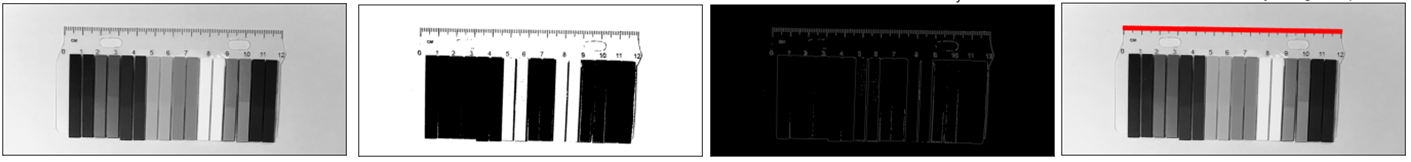
\includegraphics[width=4.5in]{FigRef.png}
    \caption{Referenzobjekt $R$. Von links nach rechts: Originalaufnahme (in Grauwerte Konvertiert), Bild nach Binarisierung, Bild nach Canny-Edge Algorithmus, detektierte Referenzlinie auf Originalbild projiziert.}
    \label{fig:fig1}
\end{figure}

\subsubsection{Binarisierung}

Das Bild wurde zunächst mit einem Schwellwert von 170 binarisiert. Der Schwellwert wurde empirisch gewählt, oder hätte durch die Analyse des Histogramms geschätzt werden können. Im Histogramm hätte man hierbei nach Tälern zwischen zwei lokalen Maxima gesucht, welche Vordergrundpixel (Lineal) und Hintergrundpixel voneinander trennen. Durch die vielen Graustufen in diesem Bild war ein empirisches Aussuchen des Schwellwertes für die Binarisierung praktikabler.

Die Binarisierung hatte zwei Gründe. Erstens sollte der uns interessierende Kontrast zwischen Bild und Hintergrund geschärft werden, und dadurch sollte die zu messende Kante des Objektes im nächsten Schritt besser detektiert werden können. Versuche haben gezeigt, dass ohne diesen Schritt die Kantendetektion nicht zu dem gewünschten Ergebnis geführt hat.

\subsubsection{Kantendetektion \/ Canny-Edge}

Anschließend sollten alle Kanten im Bild detektiert werden. Hierzu wurde der Canny-Edge Algorithmus \textit{[Cann86]} verwendet. Der Canny-Edge Algorithmus kombiniert verschiedene Faltungsoperationen \textit{[OpenCV]} und liefert ein Bild, welches lediglich Kanten mit der Breite 1 Pixel enthält. Der Canny-Edge Algorithmus benötigt ebenfalls 2 Schwellwerte. Diese wurden aus den Helligkeitswerten des Bildes geschätzt, indem zunächst der Median der Helligkeitswerte bestimmt wird, und anschließend ein Fenster um den Median mit einem definierten Parameter $\sigma$ festgelegt wurde, in welchem die Gradienten der Grauwertunterschiede liegen sollen. Die Schwellwerte hätten in diesem Bild auch manuell bestimmt werden können, erleichterten jedoch die Verarbeitung möglicher Testbilder $P_{i}$. Als Ergebnis erhalten wir Kanten der Breite 1 Pixel.

\subsubsection{Houghlines}
\label{hough}

Ziel dieses Schrittes ist es, Koordinatenpunkte von Kanten im Bild zu generieren. Die Implementierung des Hough-Algorithmus \textit{[MGK00]} in \textit{OpenCV} \emph{houghlinesp()} erkennt gerade Linien in einem Bild und berechnet deren Start- $(x_{1}, y_{1})$ und Endpunkte $(x_{2}, y_{2})$ in einem kartesischen Koordinatensystem. Dabei wurden empirisch zwei Parameter definiert, welche $(i.)$ die minimale Länge einer Linie $minlen$ in Pixel und $(ii.)$ die maximale tolerierte Lücke in einer Linie in Pixel $maxgap$ festlegen. Hier wurde sich für $minlen = 700px$ und $maxgap = 30px$ entschieden.

\subsubsection{Längenberechnung und Berechnung des Umrechnungsfaktors}
\label{laengenber}
Im nächsten Schritt wurden die Längen $l_{i}$ der Linien bestimmt. Hier wurde durch den Satz des Pythagoras
$l_{i} = \sqrt{ (x_{i,2}-x_{i,1})^{2} + (y_{i,2}-y_{i,1})^{2} }$
alle Längen $l_{i}$ berechnet. Anschließend wurde die längste Linie in $R$ als Referenzlinie bestimmt, von welcher wir die tatsächliche Länge von $120mm$ bereits kennen. Durch den Zusammenhang $\frac{analog\ gemessene\ Laenge\ |\ mm}{digital\ gemessene\ Laenge\ |\ px} = \frac{1\ mm}{1\ px}$ erhalten wir einen Umrechnungsfaktor $u$, welchen wir nun für die Längenberechnung von $P_{i}$ verwenden können. In diesem  Fall war die längste Linie (Abb. \ref{fig:fig1}) $1655px$ lang, was den $120mm$ entspricht. Dadurch erhalten wir einen Umrechnungsfaktor von etwa $u = 0,07 mm / px $.

\subsection{Verarbeitung der Testobjekte $P_{i}$}

Da wir durch unser Referenzobjekt den Umrechnungsfaktor erhalten haben, können wir im Folgenden die Testobjekte $P_{1}$ und $P_{2}$ vermessen.

\subsubsection{Vermessung von $P_{1}$}

\begin{figure}
    \centering
    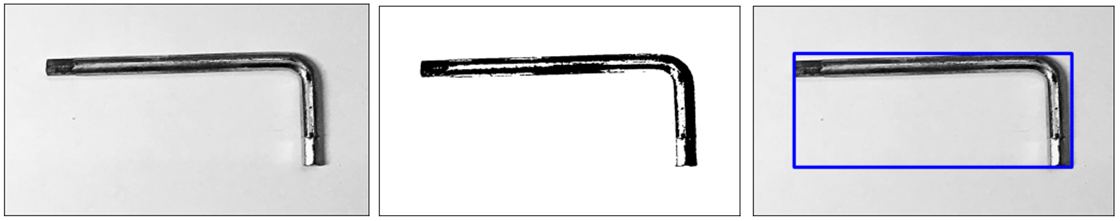
\includegraphics[width=4.5in]{FigProbe1.png}
    \caption{Testobjekt $P_{1}$. Von links nach rechts: Originalaufnahme (in Grauwerte Konvertiert), Bild nach Binarisierung, berechnete Bounding Box auf Originalbild projiziert.}
    \label{fig:fig2}
\end{figure}


Zunächst binarisieren wir $P_{1}$ mit einer Grauwertschwelle von $150$ (Abb. \ref{fig:fig2}). In einem ersten Versuch wurde - analog zur Verarbeitung von $R$ - der Canny-Algorithmus und anschließend die Funktion \textit{houghlinesp()} verwendet. Durch die spiegelnden Oberflächen und leichte Schattenwürfe von dem Objekt, war es hier schwierig, eine Linie zu finden, welche die Länge des gesamten Objektes repräsentiert. Folglich wurde hier alternativ eine Vermessung über eine Bounding Box versucht. Dazu wurde die Funktion \textit{findContours()} verwendet, welche rechteckige Umrandungen um Teilobjekte eines Bildes sucht. Die Kanten der Bounding Boxes sollten hierbei parallel zu X- und Y-Achsen des Bildes verlaufen. Die Vermessung der längsten Kante erfolgte anschließend über den oben berechneten Umrechnungsfaktor. Die Länge wurde als $65mm$ bestimmt, was auch in etwa einer analogen Messung entspricht.

\subsubsection{Vermessung von $P_{2}$}

\begin{figure}
    \centering
    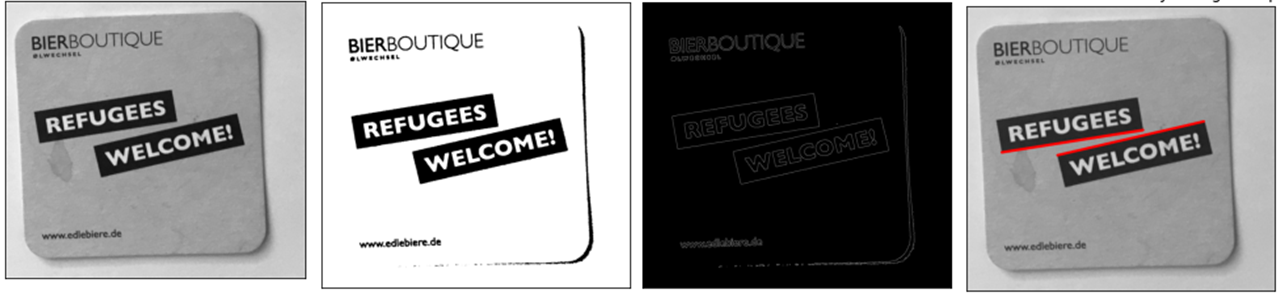
\includegraphics[width=4.5in]{FigProbe2.png}
    \caption{Testobjekt $P_{2}$. Von links nach rechts: Originalaufnahme (in Grauwerte Konvertiert), Bild nach Binarisierung, Bild nach Canny-Edge Algorithmus, zu vermessende Linien auf das Originalbild projiziert.}
    \label{fig:fig3}
\end{figure}


Die Vorverarbeitung ähnelt der von $R$. Testobjekt $P_{2}$ hat abgerundete äußere Kanten. Das Objekt wurde jedoch ausgewählt, um die Kanten des Schriftzuges zu vermessen, welcher in der Mitte von $P_{2}$ liegt. Zunächst wurde binarisiert (Schwellwert von 120), der Canny-Edge Algorithmus und schließlich die \textit{houghlinesp()} Funktion mit den Parametern $minlen = 500px$ und $maxgap = 25px$. In diesem Objekt wurden von \textit{houghlinesp()} viele Linien entdeckt, welche sich gegenseitig überlagern. Dies erschwert die Berechnung der Länge, da, selbst wenn wir die längste Linie von mehreren sich überlagernden Linien anschauen, könnte diese nicht die gesamte Länge der Kante abdecken. Aus diesem Grund entschied ich mich dazu, Linien die exakt parallel verlaufen (Toleranz von $2^{\circ}$), zu löschen, und nur die längste Linie zu behalten und zu vermessen. Hierzu berechnete ich aus den Koordinaten der Linien den dazugehörigen Winkel $\alpha = \arctan(\frac{y2-y1}{x2-x1})$, und löschte alle außer der längsten Linie mit einem bestimmten Winkel. Der Trick funktionierte in dem Fall, weil ich hier nicht an allen Linien eines parallel verlaufenden Objektes interessiert war, sondern an den Längen von zwei Schriftzügen, die gewinkelt zueinander verlaufen (Abb. \ref{fig:fig3}). Die Berechnung über den Umrechnungsfaktor ergab eine Länge von $52mm$ für den oberen Schriftzug, und $56mm$ für den unteren Schriftzug. Das entspricht grob den analog gemessenen Längen von $53mm$ und $57mm$.

\section{Fazit \& Limitationen}

Die gewählten Ansätze zur Vermessung haben für die hier gewählten Beispiele funktioniert. Die Generalisierung über andere Objekte - z.B. mit komplexerem Aufbau, einer anderen Grauwertverteilung, usw. - ist nicht gegeben. Eine einfache Weiterentwicklung der hier verwendeten Verarbeitungsschritte wären automatisierte Bestimmungen der Schwellwerte, z.B. in bei der Binarisierung oder bei dem Houghlines Algorithmus, ähnlich wie hier eine automatisierte Bestimmung der Schwellwerte beim Canny-Edge Algorithmus bereits implementiert wurde (siehe \ref{hough}). In sehr engen Anwendungsszenarien könnte es jedoch funktionieren. Z.B. für die Qualitätssicherung eines Produktes, welches unter identischen Bedingungen am Ende des Produktionsprozesses fotografiert wurde, und - falls fehlerfrei produziert - ein gleiches Ergebnis der Längendetektion liefert.

Neben der fehlenden Generalisierbarkeit, sind v.a. noch die Messfehler und deren Quellen zu diskutieren. Drei wichtige Fehlerquellen sind die Perspektive des Bildes bei Aufnahme, produzierte Schatten im Bild, und entstehende Reflektionen von Oberflächen, insofern diese nicht explizit für die Modellierung des Gegenstandes verwendet werden wollen. Messfehler könnten z.B. durch wiederholte Messungen des gleichen Objektes unter leicht veränderten Bedingungen berechnet werden. Schatten könnten durch geeignete Belichtung von mehreren Seiten minimiert werden, und spiegelnde Oberflächen könnten analog vor der Ablichtung mit entspiegelnden Substanzen bearbeitet werden.

Trotz der dargestellten Limitationen hat eine Vermessung der Objekte mit  funktioniert und eignet sich in bestimmten Anwendungsszenarien als Basis für den Aufbau komplexerer Analysepipelines.

\section*{Bibliographie}

\noindent\textbf{[Brad00]} Bradski, G.: The OpenCV Library. Dr. Dobb's Journal of Software Tools. 25. p. 120-125. 2000.

\noindent\textbf{[Cann86]} Canny, J.: A computational approach to edge detection. IEEE Transactions on pattern analysis and machine intelligence. 6, p. 679-698, 1986.

\noindent\textbf{[MGK00]} Matas, J.; Galambos, C.; Kittler, J.: Robust detection of lines using the progressive probabilistic hough transform. Computer Vision and Image Understanding, 78(1), p. 119-137. 2000.

\noindent\textbf{[OpenCV]} The OpenCV Reference Manual. Edition 4.3.0. Retrieved on 15 May 2020. https://docs.opencv.org/4.3.0/ 
\end{document}